% ============================================
% 图表与几何模板 (Chart & Geometry Templates)
% 适用：坐标系、韦恩图、饼图、柱状图
% ============================================

% --------------------------------------------
% 二维坐标系
% --------------------------------------------
\begin{figure}[H]
  \centering
  \begin{tikzpicture}[scale=0.8]
    % 坐标轴
    \draw[->] (-0.5,0) -- (5,0) node[right] {$x$};
    \draw[->] (0,-0.5) -- (0,4) node[above] {$y$};
    \node at (-0.3,-0.3) {$O$};
    
    % 刻度
    \foreach \x in {1,2,3,4} {
      \draw (\x,0.1) -- (\x,-0.1) node[below] {\small \x};
    }
    \foreach \y in {1,2,3} {
      \draw (0.1,\y) -- (-0.1,\y) node[left] {\small \y};
    }
    
    % 示例图形：矩形区域
    \draw[thick, fill=blue!20] (1,1) rectangle (3,2.5);
    \node at (2,1.75) {区域A};
    
    % 示例点
    \filldraw (4,3) circle (2pt) node[right] {$P(4,3)$};
  \end{tikzpicture}
  \caption{二维坐标系示意图}
  \label{fig:coordinate_system}
\end{figure}

% --------------------------------------------
% 韦恩图（集合关系）
% --------------------------------------------
\begin{figure}[H]
  \centering
  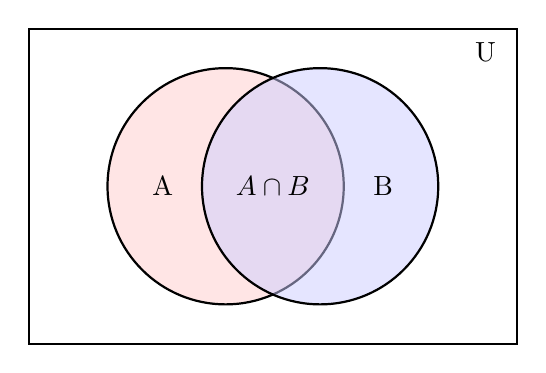
\begin{tikzpicture}
    % 集合圆
    \draw[thick, fill=red!20, fill opacity=0.5] (0,0) circle (1.5cm);
    \draw[thick, fill=blue!20, fill opacity=0.5] (1.2,0) circle (1.5cm);
    
    % 标签
    \node at (-0.8,0) {A};
    \node at (2,0) {B};
    \node at (0.6,0) {$A \cap B$};
    
    % 全集边框
    \draw[thick] (-2.5,-2) rectangle (3.7,2);
    \node at (3.3,1.7) {U};
  \end{tikzpicture}
  \caption{集合 A 与 B 的关系}
  \label{fig:venn_diagram}
\end{figure}

% --------------------------------------------
% 饼图
% --------------------------------------------
\begin{figure}[H]
  \centering
  \begin{tikzpicture}
    % 扇形数据：角度, 颜色, 标签, 百分比
    \foreach \angle/\col/\lab/\per [remember=\angle as \last (initially 0)] in {
      120/red!60/类别A/33\%,
      90/blue!60/类别B/25\%,
      80/green!60/类别C/22\%,
      70/orange!60/类别D/20\%
    } {
      \fill[\col] (0,0) -- (\last:2) arc (\last:\last+\angle:2) -- cycle;
      \node at ({\last+\angle/2}:1.3) {\small \lab};
      \node at ({\last+\angle/2}:2.5) {\small \per};
    }
  \end{tikzpicture}
  \caption{数据分布饼图}
  \label{fig:pie_chart}
\end{figure}

% --------------------------------------------
% 柱状图
% --------------------------------------------
\begin{figure}[H]
  \centering
  \begin{tikzpicture}[scale=0.9]
    % 坐标轴
    \draw[->] (0,0) -- (7,0) node[right] {类别};
    \draw[->] (0,0) -- (0,5) node[above] {数值};
    
    % Y轴刻度
    \foreach \y in {1,2,3,4} {
      \draw (-0.1,\y) -- (0.1,\y);
      \node[left] at (0,\y) {\small \y 0};
    }
    
    % 柱子
    \fill[blue!60] (1,0) rectangle (1.8,3);
    \fill[red!60] (2.5,0) rectangle (3.3,4.2);
    \fill[green!60] (4,0) rectangle (4.8,2.5);
    \fill[orange!60] (5.5,0) rectangle (6.3,3.8);
    
    % X轴标签
    \node at (1.4,-0.4) {\small Q1};
    \node at (2.9,-0.4) {\small Q2};
    \node at (4.4,-0.4) {\small Q3};
    \node at (5.9,-0.4) {\small Q4};
  \end{tikzpicture}
  \caption{季度数据柱状图}
  \label{fig:bar_chart}
\end{figure}
